\documentclass[a4paper,11pt]{article}

% ---------- Кодировка и язык ----------
\usepackage[utf8]{inputenc}
\usepackage[T2A]{fontenc}
\usepackage[russian,english]{babel}

% ---------- Геометрия страницы ----------
\usepackage[margin=2.5cm]{geometry}

% ---------- Математика ----------
\usepackage{amsmath,amssymb,amsthm,mathtools}
\usepackage{bm}          % жирные символы в формулах: \bm{x}

% ---------- Картинки ----------
\usepackage{graphicx}
\graphicspath{{figures/}}   % картинки лежат в latex/figures/
\usepackage{float}          % позиция [H] для картинок
\usepackage{subcaption}     % несколько картинок рядом

% ---------- Оформление ----------
\usepackage{enumitem}
\usepackage{booktabs}       % красивые таблицы
\usepackage{xcolor}
\usepackage[colorlinks=true,linkcolor=blue,urlcolor=blue,citecolor=blue]{hyperref}
\usepackage{cleveref}       % \cref{...} для умных ссылок

% ---------- Теоремы и окружения ----------
\theoremstyle{plain}
\newtheorem{theorem}{Теорема}[section]
\newtheorem{lemma}[theorem]{Лемма}
\newtheorem{proposition}[theorem]{Утверждение}
\newtheorem{corollary}[theorem]{Следствие}

\theoremstyle{definition}
\newtheorem{definition}[theorem]{Определение}
\newtheorem{example}[theorem]{Пример}

\theoremstyle{remark}
\newtheorem*{remark}{Замечание}

% ---------- Полезные макросы ----------
\newcommand{\R}{\mathbb{R}}
\newcommand{\Z}{\mathbb{Z}}
\newcommand{\N}{\mathbb{N}}
\newcommand{\Cx}{\mathbb{C}}   % \C занят babel-russian
\newcommand{\Tau}{\mathcal{T}} % тайлинг
\newcommand{\norm}[1]{\left\lVert #1 \right\rVert}
\newcommand{\abs}[1]{\left\lvert #1 \right\rvert}
\newcommand{\set}[1]{\left\{ #1 \right\}}
\DeclareMathOperator{\argmin}{arg\,min}
\DeclareMathOperator{\argmax}{arg\,max}

% Заметка на полях / TODO
\newcommand{\todo}[1]{\textcolor{red}{\textbf{TODO:} #1}}

\begin{document}
\section{Заметки}
\begin{definition}[Неоклассические Функции]
    Пусть $n\in\mathbb{N}$
    Будем называть функцию $f:\mathbb{R}_+^n\to\mathbb{R}_+$ \textit{неоклассической}, если она \textit{непрерывна}, \textit{вогнута} и однородна степени~1.\\
    Будем обозначать класс неоклассических функций $n$ переменных как $\Phi_n$.
\end{definition}

\begin{definition}
    Пусть $\{\hat p_t \in \mathbb{R}^{2}_{++}\}_{t\in[T]}$ --- некоторый конечный набор цен.
    Будем говорить, что вектор выпусков $y\in\mathbb{R}^{T}_{++}$ выполним при этих ценах, если
    существует такая неоклассическая функция $h\in\Phi_{2}$ и такие окрестности
    $\{U_t\ni\hat p_t\}_{t\in[T]}$, что для каждого набора $\{p_t\in U_t\}_{t\in[T]}$
    существует полная неотрицательная абсолютно непрерывная мера $\mu$ на $\mathbb{R}^{2}_{+}$, что $\forall t\in[T]\Rightarrow\mu(A_t)=y_t$, где $A_t=\{x\in\mathbb{R}^{2}_{++}\mid h(p_t\circ x)<1\}.$
\end{definition}

\begin{proposition}
    $\exists q\in conv\{p_{1},p_{3}\}:q\leq p_{2}\Rightarrow A_{2}\subset A_{1}\cup A_{3}$.
\end{proposition}

\begin{example}
    При ценах $\{\hat{p}_{1} = (4, 1), \hat{p}_{2} = (3, 3), \hat{p}_{3} = (1, 4)\}$ вектор выпусков $y=(1, 5, 3)$ не выполним.
    Более того, для случая $CES$ функций, критическая эластичность замещения $\rho_{crit}\approx -2$, а значит ромбический тайлинг будет иметь вид $\lambda$-гекса независимо от эластичности замещения. Вектору выпусков $y=(1, 5, 3)$ соответствует змейка $(0,\xi_{2},\xi_{2}+\xi_{3},\xi_{1}+\xi_{2}+\xi_{3})$ которая лежит внутри зоногона $Z_{3}$ но не содержится в $\lambda$-гексе. 
\end{example}

\begin{remark}
    Кажется, для $T=3$ не существует примера, для которого переход от $CES$ функций к неоклассическим дал бы больше выполнимых случаев.
\end{remark}

\begin{proposition} Функция $h(x):=\sqrt{x^{1}x^{2}}\exp(\frac{1}{4}\sin\ln\frac{x^{1}}{x^{2}})$ является неоклассической.
\end{proposition}

\begin{proof}
    Сначала покажем, что эта функция непрерывна на $\mathbb{R}^{2}_{+}$. Непрерывность на $\mathbb{R}^{2}_{++}$ выполнена в силу того, что $h$ представима как композиция непрерывных функций. Для того, чтобы показать непрерывность на $\partial\mathbb{R}^{2}_{+}$ заметим, что  для каждого $x\in\mathbb{R}^{2}_{++}$ значение функции $h(x)\in[e^{\frac{-1}{4}}\sqrt{x^{1}x^{2}}, e^{\frac{+1}{4}}\sqrt{x^{1}x^{2}}]$ а значит также как и в случае функций Кобба-Дугласса, наша функция продолжается по непрерывности на $\partial\mathbb{R}^{2}_{+}$ тождественным нулем.

    Теперь покажем, что эта функция вонута. Введем $u:=\ln\frac{x^{1}}{x^{2}}$, тогда гессиан имеет вид:
    \[
        \nabla^{2}h(x)
        = -\,\frac{h(x)\,\bigl(1+\sin u\bigr)\bigl(3+\sin u\bigr)}{16\,(x^{1})^{2}(x^{2})^{2}}
        \begin{pmatrix}
            (x^{2})^{2} & -x^{1}x^{2}\\[2pt]
            -x^{1}x^{2} & (x^{1})^{2}
        \end{pmatrix}.
    \]
    Множитель перед матрицей неположителен, а сама матрица имеет собственные числа $0$ и $(x^{1})^{2}+(x^{2})^{2}$, а значит сам гессиан отрицательно полуопределен и функция $h$ вогнута.
\end{proof}

\begin{example}
    Пусть $h(x)=\sqrt{x^{1}x^{2}}\exp(\frac{1}{4}\sin\ln\frac{x^{1}}{x^{2}})$ и $p\in\mathbb{R}^{2}_{++}$, тогда если выполнено неравенство $|\ln p^{1} + \ln p^{2}|<|\sin\frac{\ln p^{1} - \ln p^{2}}{2}|$ то кривые $h(x)=1$ и $h(p\circ x)=1$ имеют счетное пересечение.
\end{example}

\begin{proof}
    Введем замену координат $\theta:= \ln x^{1} + \ln x^{2}$ и $\eta := \ln x^{1} - \ln x^{2}$, в этих координатах кривая $h(x)=1$ имеет простой параметрический вид $\theta =  -\frac{\sin\eta}{2}$ и определена для любого $\eta$.

    Помимо равенства $h(x)=1$ для точки пересечения также требуется $h(x)=h(p\circ x)$.
    Полагая, что $h(x)>0$ в координатах $(\theta,\eta)$ это уравнение представимо в следующем виде:
    \[
    2\ln\frac{h(p\circ x)}{h(x)}
    = (\ln p^{1} + \ln p^{2})
    + \sin\frac{\ln p^{1} - \ln p^{2}}{2}\,\cos\left(\eta + \frac{\ln p^{1} - \ln p^{2}}{2}\right) = 0.
    \]
    Это уравнение зависит от $\theta$ и имеет $0$ корней при $|\ln p^{1} + \ln p^{2}|>|\sin\frac{\ln p^{1} - \ln p^{2}}{2}|$, континуум решений в вырожденных случаях $p = (\exp(\pi z), \exp(-\pi z))$ для $z\in\mathbb{Z}$ и счетное кол-во в остальных случаях в том числе при $|\ln p^{1} + \ln p^{2}|<|\sin\frac{\ln p^{1} - \ln p^{2}}{2}|$. Для любого $\eta$ существует единственная $\theta$, которая задает точку на $h(x)=1$, что дает счетное кол-во пересечений.
\end{proof}

\begin{example}
    Пусть неоклассическая функция имеет вид $h(x):= \sqrt{x^{1}x^{2}}\exp(G(\ln\frac{x^{1}}{x^{2}}))$, где $G(\eta) :=\tfrac{1}{10}\exp\!\left(\tfrac{-1}{\sin^{2}\eta}\right)\sin(\ctg\eta)\,\th\eta$. Пусть также $p =(\exp(\frac{\pi}{2}), \exp(\frac{-\pi}{2}))$, тогда в окрестности точки $(1,1)$ кривые $h(x)=1$ и $h(p\circ x)=1$ пересекаются счетное число раз.
\end{example}

\begin{remark}
    Важно отметить, что предыдущий пример, в котором точки пересечения
    сгущаются \emph{внутри} ортанта, не обладает свойством общего положения.
    Движение цены вдоль гиперболы $p^{1}p^{2}=1$ лишь сдвигает точку
    сгущения, но движение поперек полностью разрушает счетность числа
    пересечений. Вероятно, для цены общего положения (вопрос о корректном
    определении) сгущение пересечений возможно только в окрестности осей.
\end{remark}

\section{Башни Ромбических Тайлингов}

Зафиксируем неоклассическую функцию $h\in\Phi$ и статистику различных цен $\{p_{t}\in\mathbb{R}^{2}_{++}\}_{t\in[T]}$. Будем полагать, что кривые $h(p_{t}\circ x)=1$ пересекаются не более чем счетное число раз, все пересечения происходят трансверсально (в том числе не на осях), никакие три кривых не пересекаются в одной точке и никакие два пересечения не лежат на одной прямой с началом координат. Более того, будем полагать, что аргументы углов пересечения не сгущаются на интервале $(0,\pi/2)$. 

В таком случае аргументы точек пересечения возможно \textit{пронумеровать} целыми числами, получив последовательность углов $\dots,\alpha_{-1},\alpha_{0},\alpha_{1},\dots$. Тогда на непересекающихся интервалах $(\alpha_{z},\alpha_{z+1})$ не происходит пересечений. Зафиксируем произвольный угол $\beta_{z}\in(\alpha_{z},\alpha_{z+1})$ и определим перестановку $\sigma_{z}$, которая упорядочивала бы значения $h(p^{1}_{t}\sin\beta_{z}, p^{2}_{t}\cos\beta_{z})$ по возрастанию.

В полученной последовательности, подряд идущие перестановки отличаются перестановкой двух соседних (с точки зрения перестановки) элементов: $\sigma_{z+1} = (\sigma_{z}(i_z), \sigma_{z}(i_z+1))\circ\sigma_{z}$. Это значит, что они сравнимы по Брюа, и либо $Inv(\sigma_{z+1})\subset Inv(\sigma_{z})$, либо $Inv(\sigma_{z+1})\supset Inv(\sigma_{z})$.

Построим по последовательности перестановок двумерный клеточный комплекс:
для каждого $z$ построим по ромбическому тайлингу из одного ромба, в случае $Inv(\sigma_{z+1})\supset Inv(\sigma_{z})$ положим $\Tau_{z} = Z(\sigma_{z+1},\sigma_{z})$ и \textit{расскрасим} его единственный ромб в \textit{белый}, иначе же положим $\Tau_{z} = Z(\sigma_{z},\sigma_{z+1})$ и расскрасим ромб в \textit{черный}. Полученный тайлинг является $2$-мерным клеточным комплексом с $(T+2)$ $0$-клетками, $(T+2)$ $1$-клеткой и одной четырехугольной $2$-клеткой, покрашенной в черный или белый в зависимости от ориентации тайлинга.

Далее \textit{склеим} ромбические подряд идущие тайлинги согласовано с ориентацией.
\begin{enumerate}
    \item \textit{Белый-белый}: склеим правую змейку белого тайлинга $\Tau_{z+1} = Z(\sigma_{z+2},\sigma_{z+1})$\\
    с левой змейкой белого тайлинга $\Tau_{z} = Z(\sigma_{z+1},\sigma_{z})$.
    \item \textit{Черный-белый}: склеим левую змейку черного тайлинга $\Tau_{z+1} = Z(\sigma_{z+1},\sigma_{z+2})$\\
    с левой змейкой белого тайлинга $\Tau_{z} = Z(\sigma_{z+1},\sigma_{z})$.
    \item \textit{Белый-черный}: склеим правую змейку белого тайлинга $\Tau_{z+1} = Z(\sigma_{z+2},\sigma_{z+1})$\\
    с правой змейкой черного тайлинга $\Tau_{z} = Z(\sigma_{z},\sigma_{z+1})$.
    \item \textit{Черный-черный}: склеим левую змейку черного тайлинга $\Tau_{z+1} = Z(\sigma_{z+1},\sigma_{z+2})$\\
    с правой змейкой черного тайлинга $\Tau_{z} = Z(\sigma_{z},\sigma_{z+1})$.
\end{enumerate}

В итоге получается двумерный клеточный комплекс, представляющийиз себя обобщение ромбического тайлинга на случай множественного пересечения кривых. В них все также можно определить понятие спектра вершины, змейку или гекс. Но из-за того, что несколько различных вершин могут иметь равный спектр однозначность теряется. На данный момент мне неизвествно можно ли восстановить данную структуру по мультимножеству, в котором будет известно сколько вершин обладает конкретным спектром.

\begin{figure}[H]
    \centering
    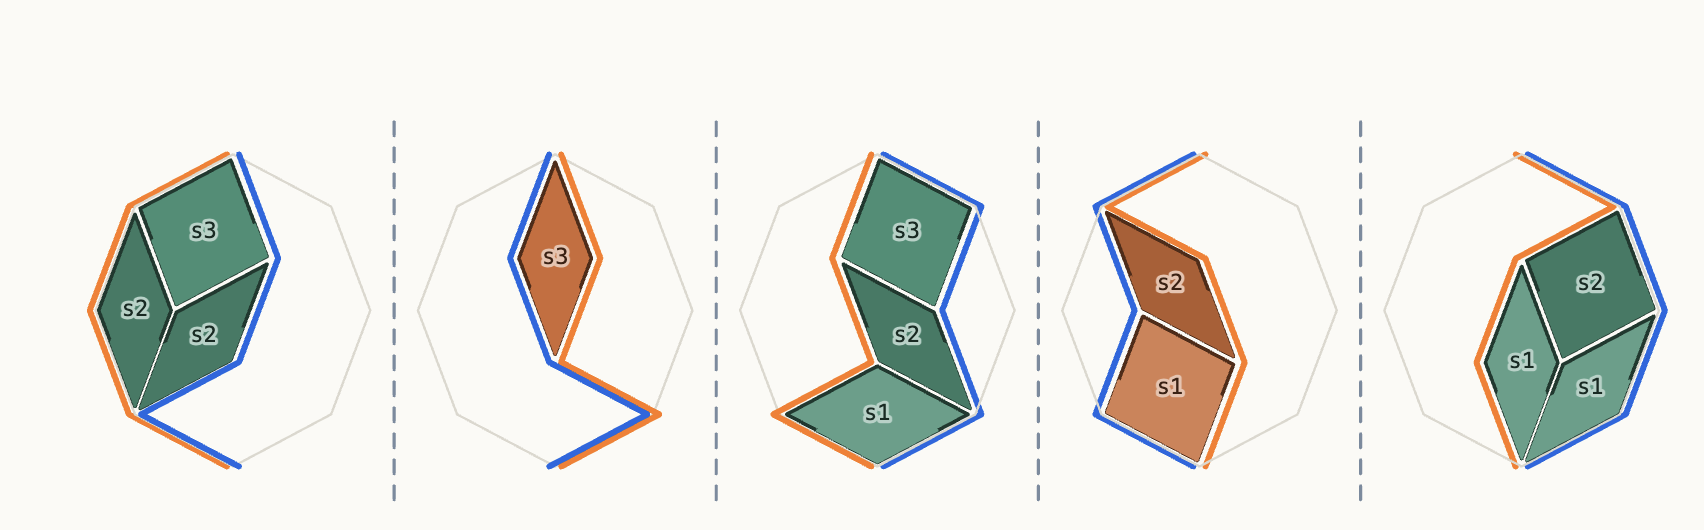
\includegraphics[width=\textwidth]{tower_gluing.png}
    \caption{Клеточный комплекс из ромбических тайлингов: подряд идущие тайлинги, склеенные согласованно с ориентацией. Этой структуре соовтетствует слово $s_2 s_3 s_2 s_3 s_1 s_2 s_3 s_1 s_2 s_1 s_2 s_1$}
    \label{fig:tower_gluing}
\end{figure}

В данной структуре, как и в ромбических тайлингах, встречаются гексы. И деформации кривых позволяют совершить аналогичный флип, причем необязательно все ромбы должны иметь один цвет. Ниже приведен пример такого \textit{разноцветного} флипа.

\begin{figure}[H]
    \centering
    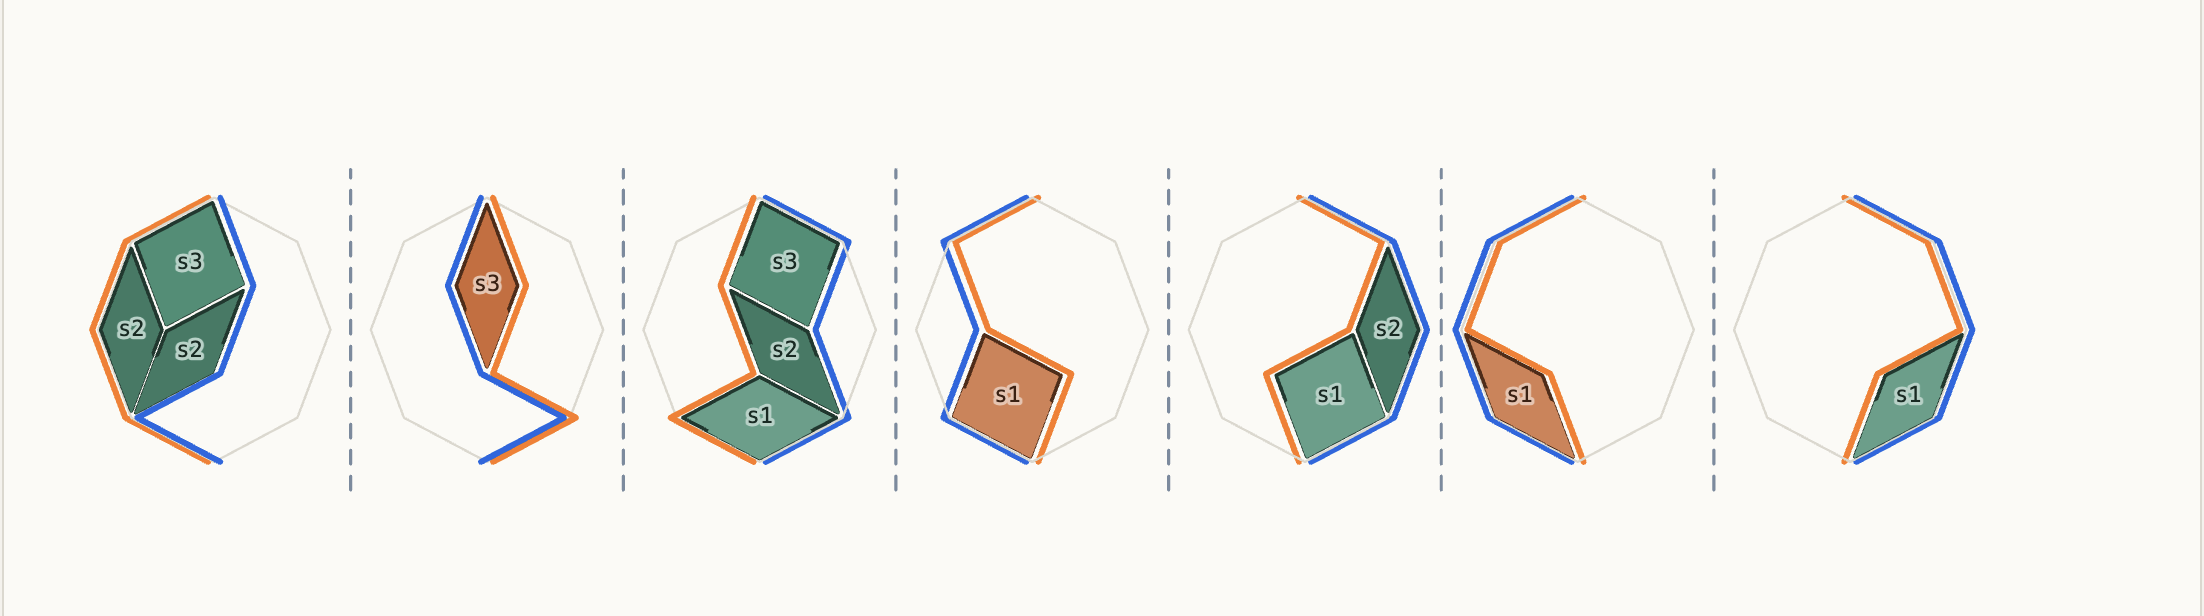
\includegraphics[width=\textwidth]{tower_gluing_2.png}
    \caption{На данном рисунке изображена структура, полученная из структуры предыдущего рисунка повышающим флипом $s_1 s_2 s_1\to s_2 s_1 s_2$, при этом соответствующие ромбы сохраняют свой цвет. Этой структуре соответствует слово $s_2 s_3 s_2 s_3 s_1 s_2 s_3 s_1 s_1 s_2 s_1 s_1$.}
    \label{fig:colored_flip}
\end{figure}

Помимо привычного флипа, для клеточных комплексов существует специфичное преобразование: \textit{рождение/аннигиляция} двух ромбов разного цвета. Причем если для удаления последовательность цветов неважна, то для рождения они должны быть согласованы с остальным комплексом.

\begin{figure}[H]
    \centering
    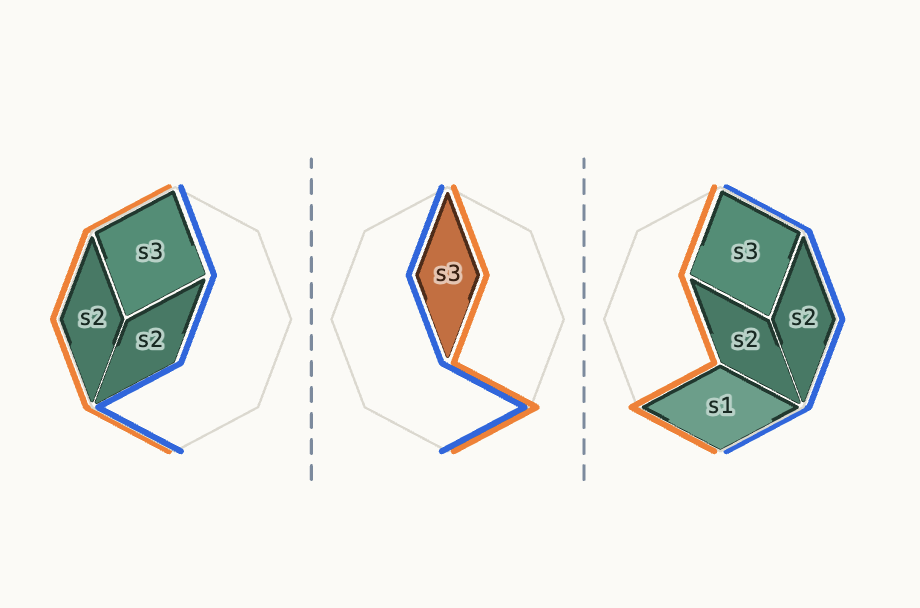
\includegraphics[width=0.5\textwidth]{annihilation.png}
    \caption{Аннигиляция двух пар ромбов $s_1 s_1$ разного цвета в структуре с предыдущего рисунка. Полученной структуре соответствует слово $s_2 s_3 s_2 s_3 s_1 s_2 s_3 s_2$.}
    \label{fig:annihilation}
\end{figure}

\begin{figure}[H]
    \centering
    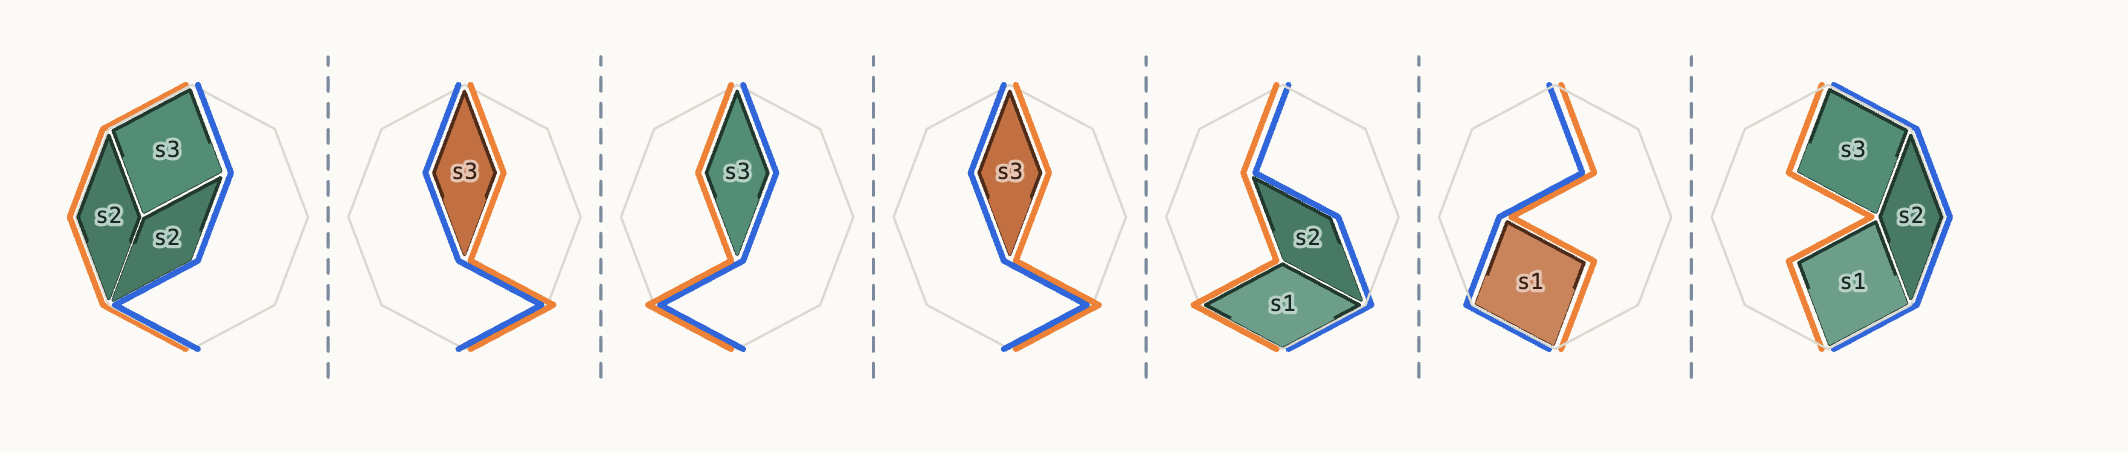
\includegraphics[width=\textwidth]{birth.png}
    \caption{Рождение пар ромбов в структуре с предыдущего рисунка: пары $s_3 s_3$ и $s_1 s_1$ рождаются как черно-белая либо как бело-черная в зависимости от того, как раскрашен остальной комплекс.}
    \label{fig:birth}
\end{figure}

\begin{figure}[H]
    \centering
    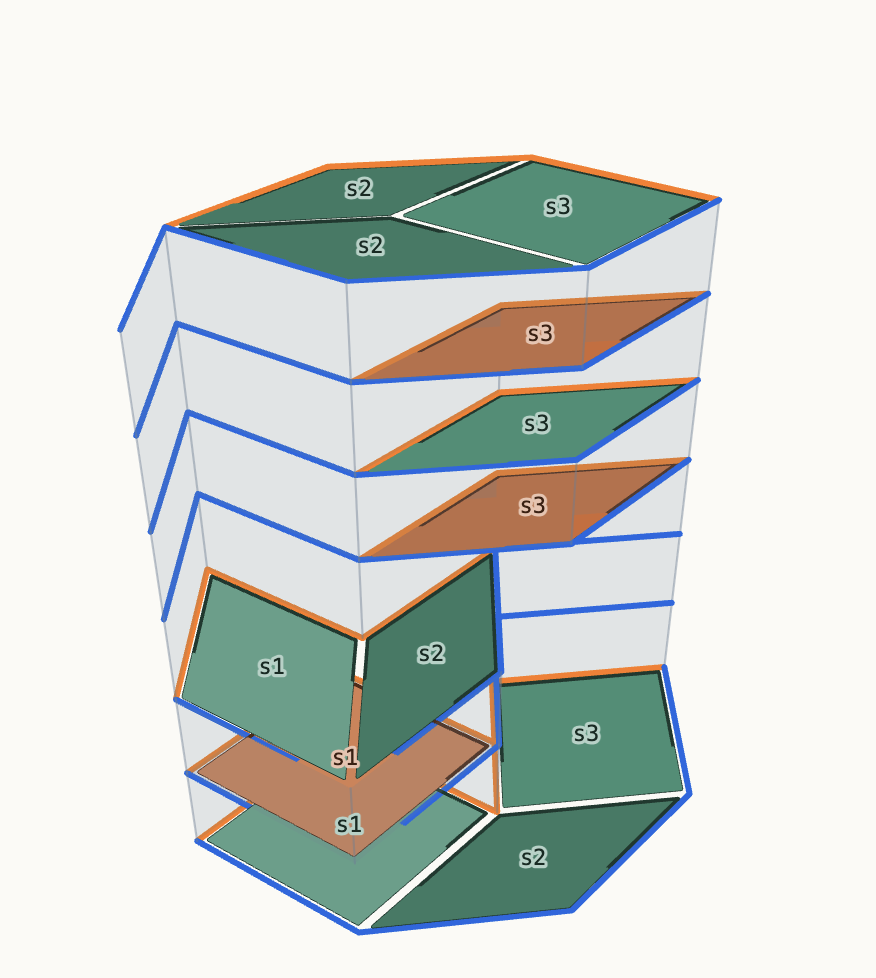
\includegraphics[width=0.35\textwidth]{tower_3d.png}
    \caption{Башня ромбических тайлингов с предыдущего рисунка, изображенная целиком: тайлинги $\Tau_z$ расположены друг над другом и склеены по змейкам.}
    \label{fig:tower_3d}
\end{figure}

Помимо конечных клеточных комплексов могут получаться и бесконечные. Одним из примеров таких структур можно рассмотреть пример счетного пересечения в общем положении. При \textit{расцеплении} счетное число пересечений превращается в ноль, и аннигилируется сразу счетное число ромбов. Более интересным примером является ситуация, когда имеется три кривых в общем положении, которые попарно пересекаются счетное число раз.

\begin{figure}[H]
    \centering
    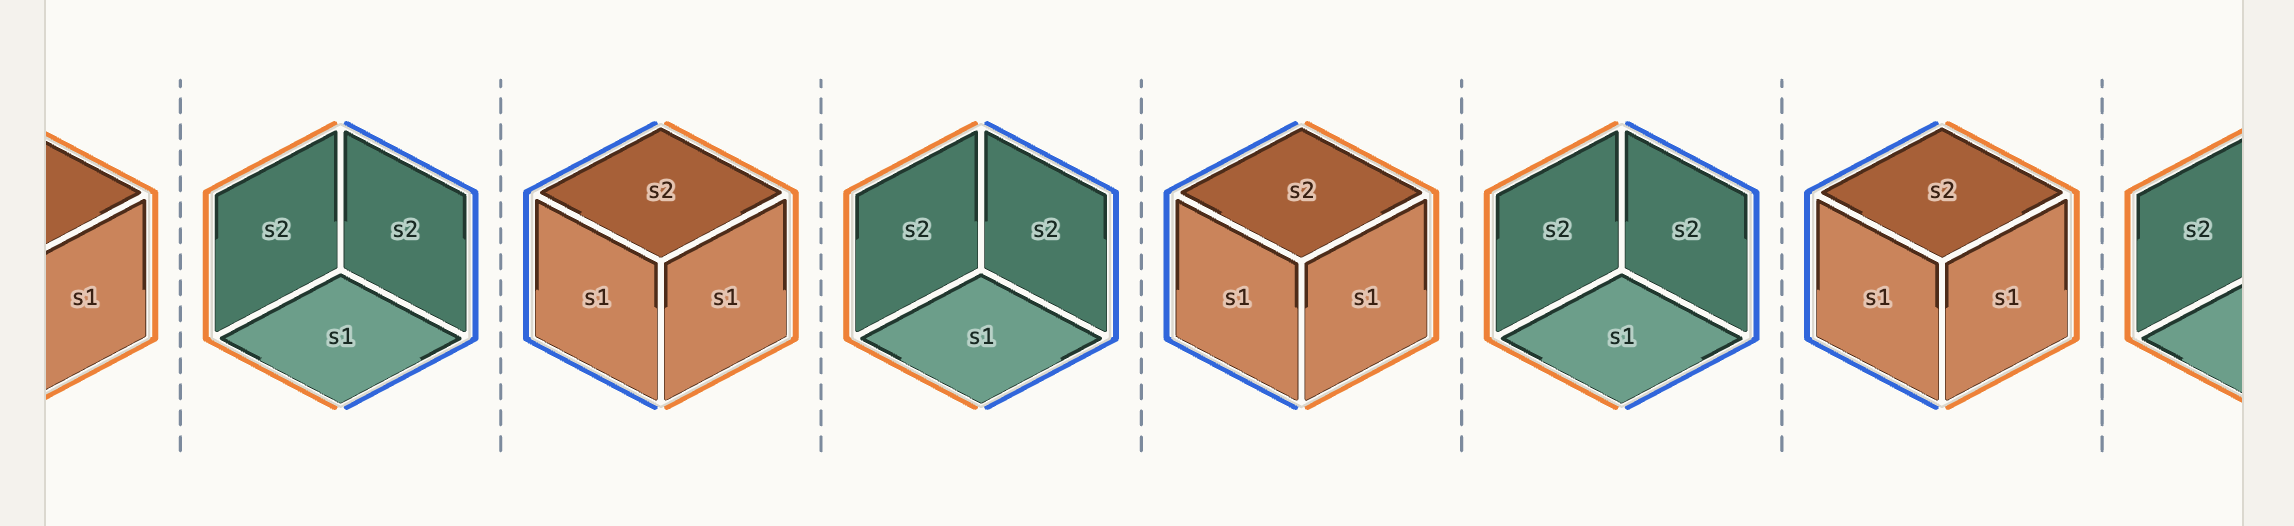
\includegraphics[width=\textwidth]{infinite_complex.png}
    \caption{Фрагмент бесконечного клеточного комплекса для трех кривых, попарно пересекающихся счетное число раз: белые и черные гексы $s_2 s_1 s_2$ и $s_1 s_2 s_1$ чередуются, и структура продолжается неограниченно в обе стороны.}
    \label{fig:infinite_complex}
\end{figure}

\begin{figure}[H]
    \centering
    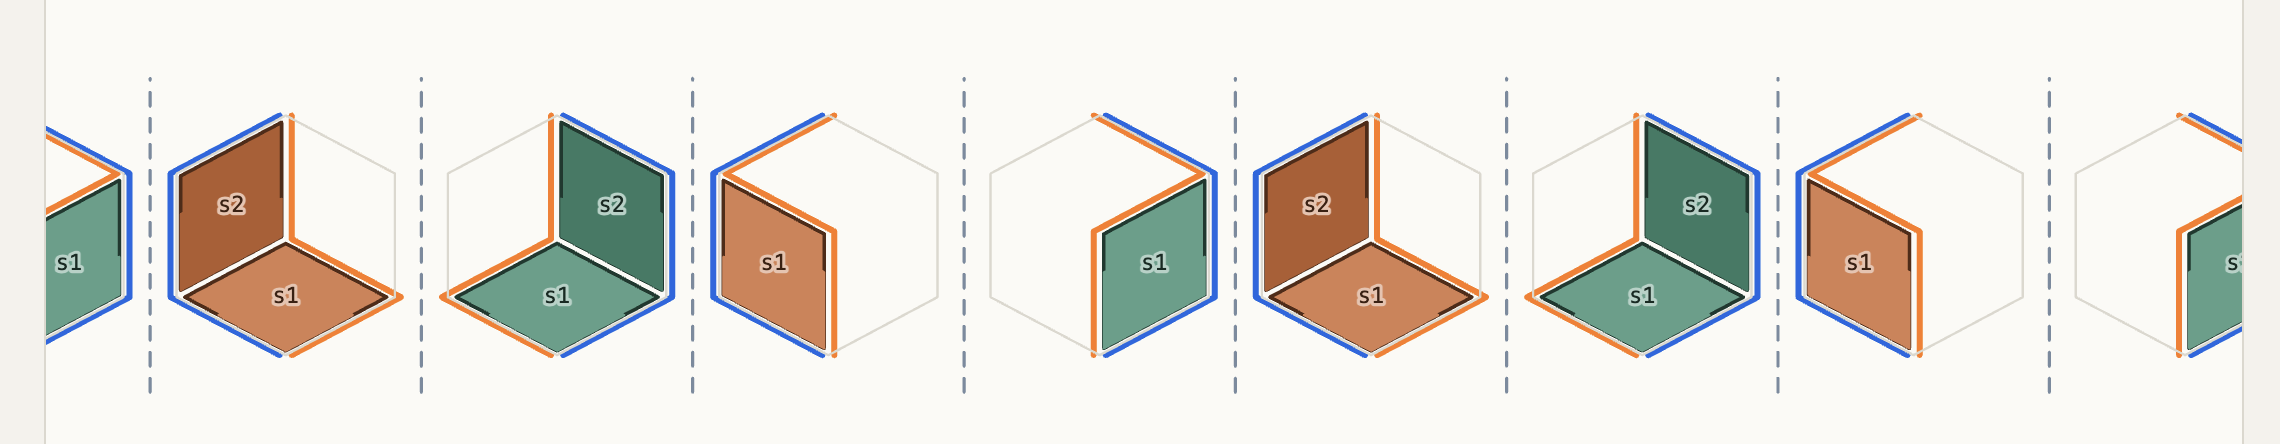
\includegraphics[width=\textwidth]{infinite_flip.png}
    \caption{Расцепление первой и третьей кривых в комплексе с предыдущего рисунка: флип произошел у каждого второго гекса, причем не в пределах одноцветного слоя-тайлинга, а через границу между слоями.}
    \label{fig:infinite_flip}
\end{figure}

\begin{figure}[H]
    \centering
    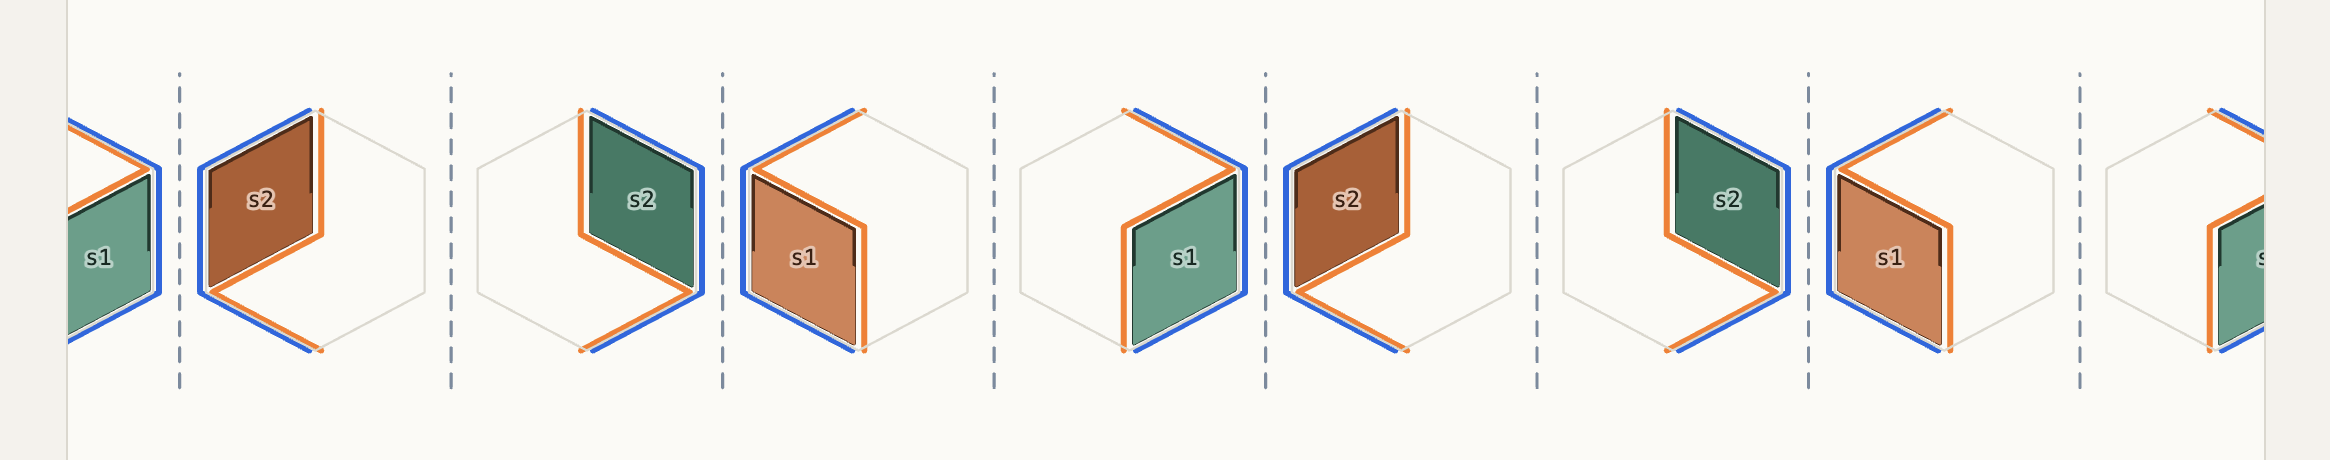
\includegraphics[width=\textwidth]{infinite_annihilation.png}
    \caption{Комплекс после расцепления первой и третьей кривых: часть ромбов аннигилировала, и остались только ромбы, отвечающие счетному пересечению первой и второй кривых и счетному пересечению второй и третьей.}
    \label{fig:infinite_annihilation}
\end{figure}

\begin{figure}[H]
    \centering
    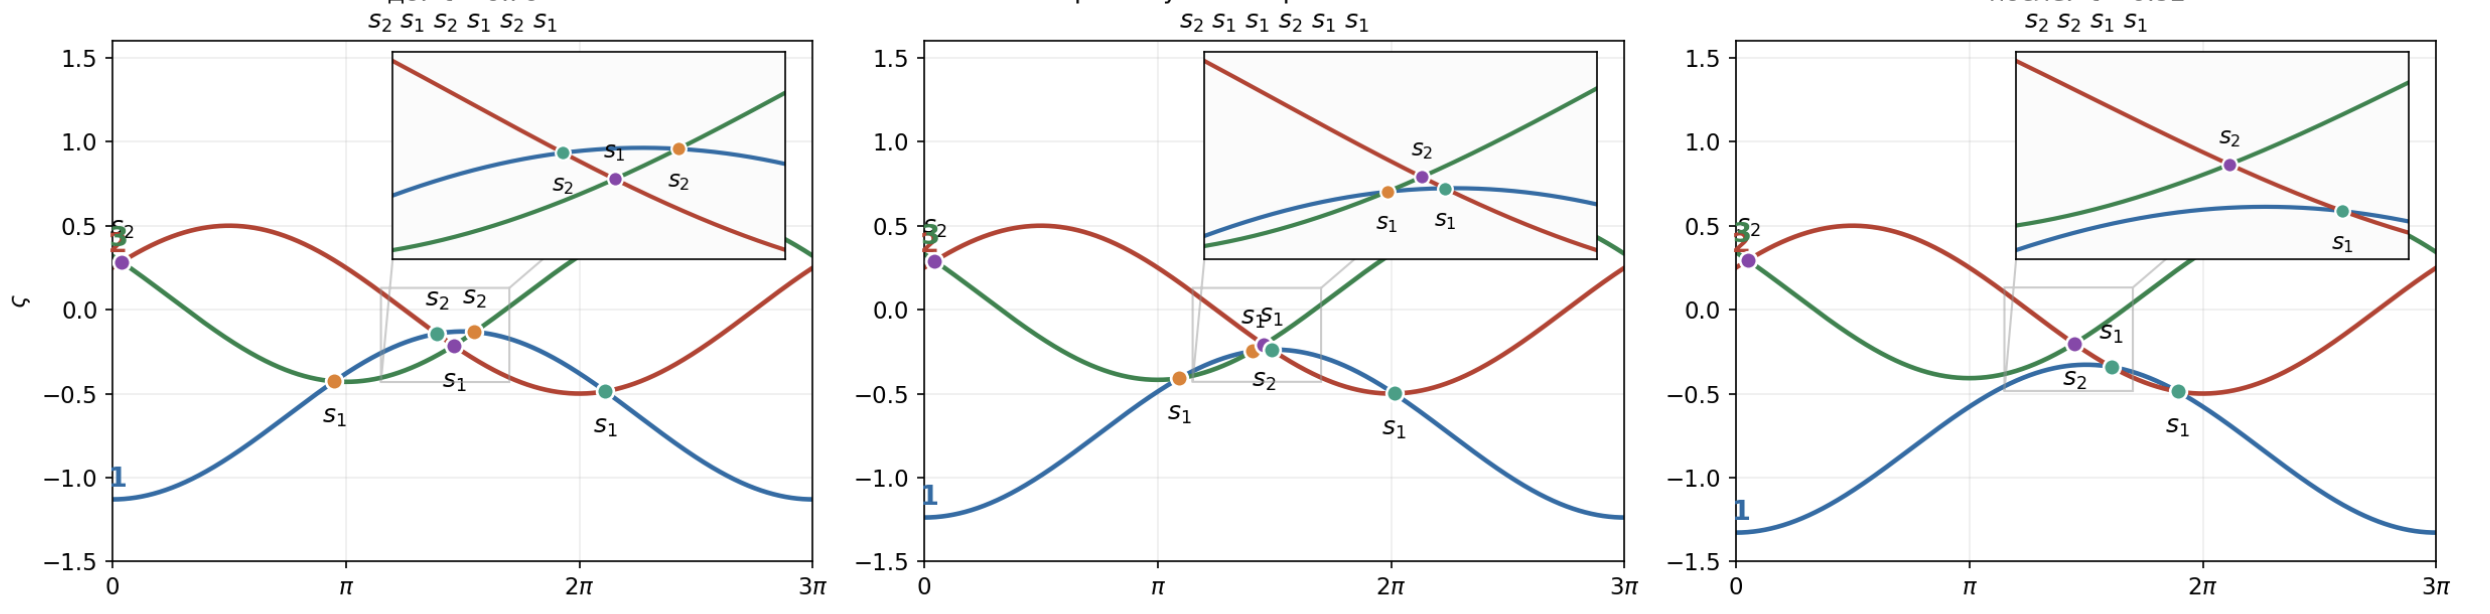
\includegraphics[width=\textwidth]{periodic_curves.png}
    \caption{Периодическая часть трех кривых для трех рассмотренных случаев и соответствующие им слова: $s_2 s_1 s_2 s_1 s_2 s_1$ (все три пары пересекаются), $s_2 s_1 s_1 s_2 s_1 s_1$ (после флипа через границу) и $s_2 s_2 s_1 s_1$ (после аннигиляции, остались пересечения $1$--$2$ и $2$--$3$).}
    \label{fig:periodic_curves}
\end{figure}

В рассматриваемых случаях клеточные комплексы, пусти и были бесконечно большими, все равно периодически повторялись, что позволяло рассматривать их как конечные. Неясно возможно ли создать с помощью неоклассических функций какие-либо \textit{иррациональные} или \textit{трансцендентные} (в смысле условия Лиувилля) последовательности

\end{document}
